\documentclass[addpoints]{exam}

\usepackage{graphicx}
\usepackage{hyperref}
\usepackage{tabularx}

\graphicspath{{images/}}

% Header and footer.
\pagestyle{headandfoot}
\runningheadrule
\runningfootrule
\runningheader{CS 440}{Project I: Flight Simulator}{Fall 2020}
\runningfooter{}{Page \thepage\ of \numpages}{}
\firstpageheader{}{}{}

\qformat{{\large\bf \thequestion. \thequestiontitle}\hfill}
\boxedpoints

\title{Project I: Flight Simulator}
\author{CS 440 Computer Graphics\\Habib University\\Fall 2020}
\date{Due: 2359h on Friday, 13 November}

\begin{document}
\maketitle
\thispagestyle{empty}

In this project you will implement a flight simulator. High level instructions are provided and you are expected to use your knowledge of math, computer science, and computer graphics to make reasonable implementation decisions. This is a complicated task and is broken down for you in the following sequence of problems. Use your judgment to put the individual pieces together. Make use of the discussion avenues specified in this project's README as needed.

Note that the illusion of flight is to be achieved by varying cameras parameters, not by transforming geometry.

The simulator should run in a page titled `simulator.html`.

\begin{questions}

  %%%%%%%%%%%%%%%%%%%%%%%%%%%%%%%%%%%%%%%%%%%%%%%%%%
  \titledquestion{Plain Terrain}

  A \textit{height map} is commonly used to generate a \textit{terrain mesh}. A height map is a function that takes in 2 values, e.g. longitude and latitude, and generates a height value, $h$. Write a function to generate a height field over a given area in the $xz$- plane. The function would generate a grid in the given area, triangulate it, and randomly perturb the $y$ coordinate of the grid points within $(-2, 2)$.
  \begin{figure}[!h]
    \centering
    \begin{tabular}{cc}
      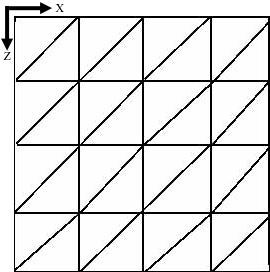
\includegraphics[height=.35\textwidth]{terrain1}
      & 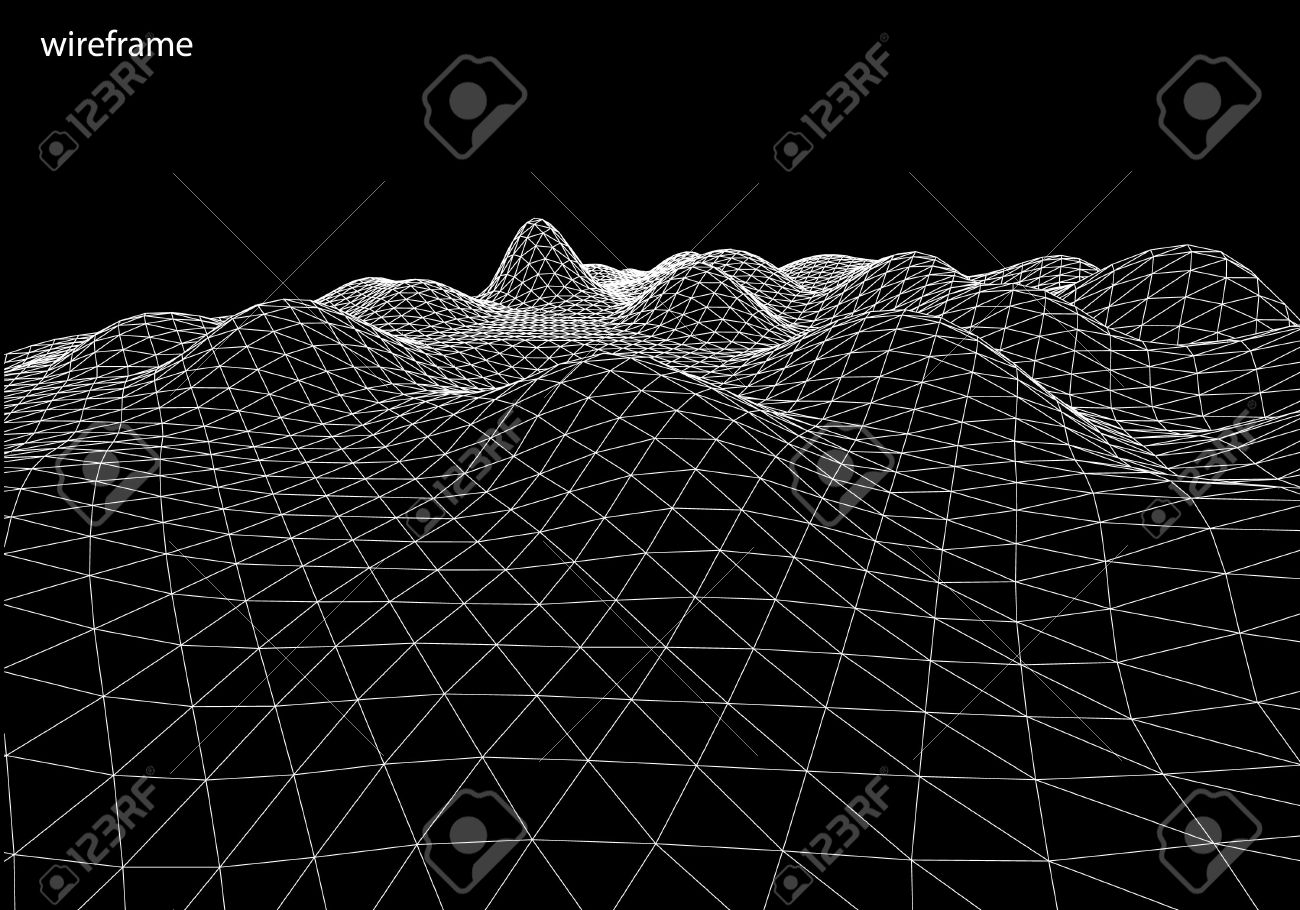
\includegraphics[height=.35\textwidth]{terrain2}\\
      (a) & (b)
    \end{tabular}
    \caption{(a) A triangulated grid in the $xz$- plane. (from \href{http://keithditch.powweb.com/Games/XNA/html/xna\_terrain.html}{Toymaker}) (b) View of an example height field generated by perturbing the $y$- coordinate of the grid points. (from \href{https://www.123rf.com/photo_54102307_stock-vector-3d-wireframe-terrain-contour-vector.html}{123RF})}
  \end{figure}
  
  \noindent\underline{Implementation Tips}
  \begin{itemize}
  \item Write a function \texttt{get\_patch(xmin, xmax, zmin, zmax)} to generate a terrain patch in an appropriate format and return it.
  \end{itemize}

  %%%%%%%%%%%%%%%%%%%%%%%%%%%%%%%%%%%%%%%%%%%%%%%%%%
  \titledquestion{Flight}

  Implement a flyby view of your generated terrain. This is the perspective view obtained from a plane flying at a certain altitude (e.g. $y=3$) above your terrain and facing straight ahead, i.e. parallel to ground level. Implement mechanisms to dynamically effect the following.
    \begin{itemize}
    \item alter the bounds of the view, i.e. \textit{left}, \textit{right}, \textit{top}, \textit{bottom}, \textit{near}, and \textit{far} of the viewing volume within reasonable constraints. Use the following key map.
      \begin{itemize}
        \item \texttt{1} and \texttt{Shift+1} to vary \textit{left}.
        \item \texttt{2} and \texttt{Shift+2} to vary \textit{right}.
        \item \texttt{3} and \texttt{Shift+3} to vary \textit{top}.
        \item \texttt{4} and \texttt{Shift+4} to vary \textit{bottom}.
        \item \texttt{5} and \texttt{Shift+5} to vary \textit{near}.
        \item \texttt{6} and \texttt{Shift+6} to vary \textit{far}.
      \end{itemize}
    \item quit the simulator. Map the \texttt{Escape} key to quit..
    \end{itemize}

    \noindent\underline{Implementation Tips}
    \begin{itemize}
    \item Modifying a value beyond its allowed constraints should have no effect.
    \end{itemize}
    
  %%%%%%%%%%%%%%%%%%%%%%%%%%%%%%%%%%%%%%%%%%%%%%%%%%
  \titledquestion{Varied Terrain}

    Specify a certain height ($y=0$) in your terrain as \textit{ground level}. Your terrain contains greenery at ground level and the points are colored green. Terrain below ground level is covered by water. Only the surface of the water is visible which is colored blue. Terrain above ground level is mountainous and the points are colored green to brown to white as the height increases. Implement mechanisms to dynamically effect the following.
    \begin{itemize}
    \item toggle the view of the terrain in the circular order: its points, its wireframe, and its faces. Map the key \texttt{V} to the toggling of the view. 
    \item toggle the shading in the circular order: flat, smooth, and Phong. Map the key \texttt{C} to the toggling of the coloring scheme.
    \end{itemize}

    \noindent\underline{Implementation Tips}
    \begin{itemize}
    \item The mapping from altitude to color could use the \texttt{map\_point} function from previous assignments.
    \item The points in the \textit{points} view must be large enough to be visible.
    \item To flat shade a polygon, apply the average color of the three vertices.
    \end{itemize}

  %%%%%%%%%%%%%%%%%%%%%%%%%%%%%%%%%%%%%%%%%%%%%%%%%%
  \titledquestion{Some \href{https://en.wikipedia.org/wiki/Flight_dynamics_(fixed-wing_aircraft)}{Flight Dynamics}}

    \begin{figure}[!h]
    \centering
    \begin{tabular}{cc}
      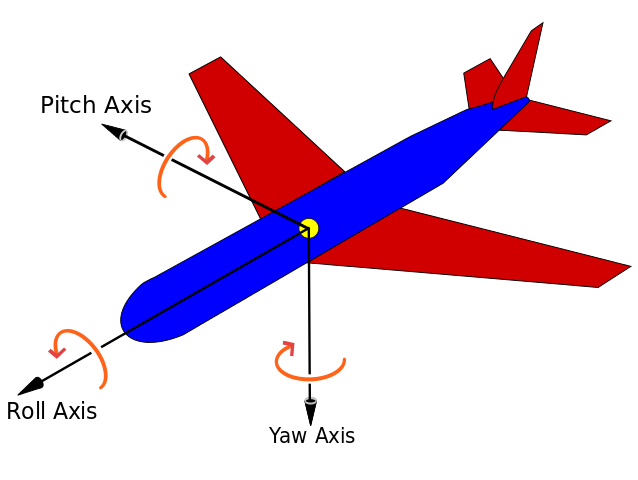
\includegraphics[height=.35\textwidth]{plane}
      &   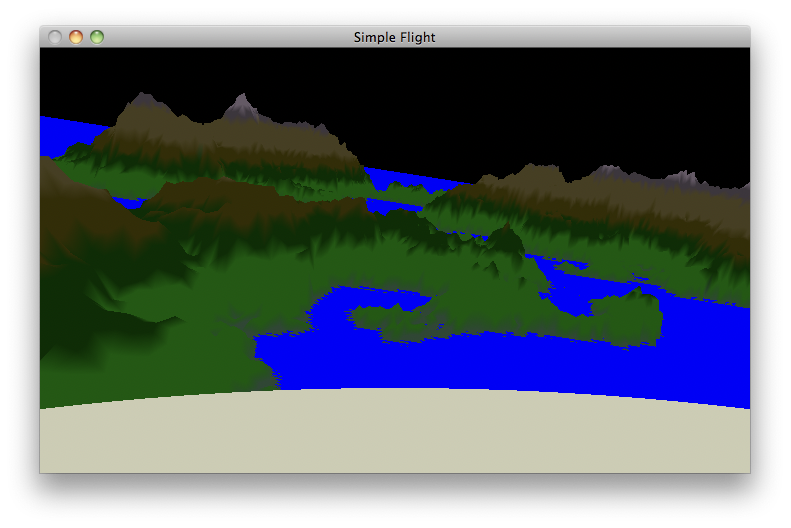
\includegraphics[height=.35\textwidth]{view}\\
      (a) & (b)
    \end{tabular}
    \caption{(a) The three rotations of a plane. (from \href{https://en.wikipedia.org/wiki/Flight_dynamics_(fixed-wing_aircraft}{Wikipedia}) (b) An example view of the terrain. Your view need not contain the dashboard.}
    \label{fig:rotate}    
  \end{figure}

  The orientation of a plane in flight is determined by its rotation about three axes. The rotations, termed \textit{pitch}, \textit{roll}, and \textit{yaw}, and the corresponding axes are illustrated in Figure \ref{fig:rotate}. Implement mechanisms to dynamically effect the following.
  \begin{itemize}
  \item each of the indicated rotations constrained to $(-90^\circ, 90^\circ)$. Use the following key map.
    \begin{itemize}
    \item \texttt{W, S} (and lower case) for pitch
    \item \texttt{A, D} (and lower case) for yaw
    \item \texttt{Q, E} (and lower case) for roll
    \end{itemize}
    Constrain the rotations to $(-90^\circ, 90^\circ)$ and the plane's altitude as appropriate, e.g. $(2.5, 3.5)$.
  \item increase and decrease the speed of the plane between $[0,S]$ where $S$ is a maximum speed of your choosing. Use the \texttt{up} and \texttt{down} arrows to vary speed.
  \end{itemize}

    \noindent\underline{Implementation Tips}
    \begin{itemize}
    \item Modifying a value beyond its allowed constraints should have no effect.
    \item You will have to infer the changes to the viewing direction, up vector, and position of the plane with each rotation.
    \item Constrained altitude means that the plane will not run aground, nor will it fly up into space. Rather, its altitude will always stay within reasonable bounds.
    \item The rotation constraints ensure that the plane will never turn so much as to travel backward.
    \item The altitude constraint ensures that the plane will not run aground, nor will it fly up into space.
    \item The speed constraint allows for the plane to stand still.
    \end{itemize}

    
  %%%%%%%%%%%%%%%%%%%%%%%%%%%%%%%%%%%%%%%%%%%%%%%%%%
  \titledquestion{To Infinity}

    As the terrain is finite, the plane will ultimately fly out of it. Modify your implementation such that a new terrain patch is dynamically computed and added when the plane approaches the boundary of the patch that it is currently flying over. This way, the plane never flies out of terrain.

    \noindent\underline{Implementation Tips}
    \begin{itemize}
    \item The more you fly, the more terrain patches will be added and the more your GPU's memory will be consumed resulting in a slowdown. To prevent this, make sure to unload previous terrains.
    \item Make sure to add appropriate patches accounting for the plane's current flight direction. 
    \item Ensure that the plane is never flying over empty terrain, no matter its speed or rotation.
    \item Instead of generating a very large terrain, load a terrain that is large enough for the current view and generate and add new terrain based on the plane's motion as it approaches the current boundary.
    \item Instead of unloading terrain, you can rewrite already allocated buffers. Making use of the fact that the flight constraints ensure that the plane will not travel backward, figure out how many patches you need to keep in memory at any given time.
    \end{itemize}
    
    %%%%%%%%%%%%%%%%%%%%%%%%%%%%%%%%%%%%%%%%%%%%%%%%%% 
  \titledquestion{Freak Out (Bonus)}
  You can include the following additional functionality for a bonus.
  \begin{itemize}
  \item The height map is not completely random but is sensitive to neighboring points thus yielding a smoother terrain.
  \item The height field is read in from an image, e.g. as described \href{http://www.cs.cmu.edu/~jkh/462_s07/assts/assignment1/}{here}.
  \item Any other desired functionality.
  \end{itemize}

\end{questions}

\end{document}
%%% Local Variables:
%%% mode: latex
%%% TeX-master: t
%%% End:
